%% ============================================================
%% PAC-Bayesian Generalization Bounds for Weight-Decomposed
%% Low-Rank Adaptation -- CS229 Project (focused 6-page report)
%% Proves Theorems 3.4, 3.10, 3.12 and verifies them empirically.
%% ============================================================
\documentclass[11pt]{article}
\usepackage[margin=1in]{geometry}
\usepackage{amsmath, amssymb, amsthm}
\usepackage{mathtools}
\usepackage{graphicx}
\usepackage{booktabs}
\usepackage{caption}
\usepackage{hyperref}
\usepackage{cleveref}

\graphicspath{{figures/}}
\setlength{\parskip}{2pt}
\captionsetup{font=small}

\newtheorem{theorem}{Theorem}[section]
\newtheorem{lemma}[theorem]{Lemma}
\newtheorem{remark}[theorem]{Remark}
\crefname{theorem}{Theorem}{Theorems}
\crefname{lemma}{Lemma}{Lemmas}

\newcommand{\KL}{\mathrm{KL}}
\newcommand{\vMF}{\mathrm{vMF}}
\newcommand{\Ad}{A_d}
\newcommand{\Ak}{A_k}
\newcommand{\Sd}{\mathbb{S}^{d-1}}
\newcommand{\Sk}{\mathbb{S}^{k-1}}
\newcommand{\N}{\mathcal{N}}
\newcommand{\E}{\mathbb{E}}
\newcommand{\R}{\mathbb{R}}
\newcommand{\Cdir}{C_{\mathrm{dir}}}
\newcommand{\Thetaglob}{\Theta_{\mathrm{global}}}

\title{\textbf{PAC-Bayesian Generalization Bounds for\\
Weight-Decomposed Low-Rank Adaptation}}
\author{Stephen Zhang \and Varun Prakash \and Soham [Surname]}
\date{\today}

\begin{document}
\maketitle
\vspace{-1.5em}

\begin{abstract}
\small
Parameter-efficient fine-tuning (PEFT) methods such as DoRA and MAP decompose weight
updates into magnitude and directional components, yet their generalization behavior
is poorly understood. We give a PAC-Bayesian analysis of weight-decomposed adaptation
using von Mises--Fisher (vMF) priors on the hypersphere, yielding closed-form KL
complexity terms in the angular deviations between pretrained and fine-tuned
directions. We prove three results and verify each on RoBERTa-base fine-tuned across
four GLUE tasks: a \emph{non-asymptotic directional KL bracket}
(\cref{thm:nonasymptotic}), valid beyond the high-concentration regime; an
\emph{angular complexity comparison} (\cref{thm:comparison}) showing that column-wise
methods (DoRA) \emph{sum} directional complexity over local angles while global
methods (MAP) \emph{average} it into a single rotation; and a \emph{sparse-regime
advantage} (\cref{thm:dora_advantage}) characterizing when each method is preferable.
Measuring per-column angles over $2592$ weight matrices, the comparison identity holds
to machine precision (and with $R^2{=}0.995$ in its measured form), the KL bracket
holds with zero violations and a $77$--$307\times$ asymptotic-to-non-asymptotic
tightening, and the effective sparsity $s/d$ cleanly separates a sparse,
DoRA-favored regime (RTE, $s/d{\approx}0.10$) from dense, MAP-favored regimes
(SST-2/QNLI/MNLI, $s/d{\ge}0.95$), as the theory predicts.
\end{abstract}

\section{Introduction}
Large models are adapted to downstream tasks by parameter-efficient fine-tuning
(PEFT), which modifies a small subset of parameters. DoRA~\cite{liu2024dora} updates
each \emph{column} of a weight matrix independently (column-wise rotations); MAP~\cite{si2025map}
rotates the entire flattened matrix as one vector. There is no theory explaining when
one generalizes better than the other. We close this gap with a PAC-Bayesian analysis:
modeling directional updates with vMF distributions on the hypersphere yields bounds
depending explicitly on angular deviations, giving a notion of \emph{directional
complexity}. We prove a non-asymptotic KL bound (\cref{thm:nonasymptotic}), an
angular comparison theorem (\cref{thm:comparison}), and a sparse-regime advantage
result (\cref{thm:dora_advantage}), and verify all three empirically on RoBERTa-base.

\section{Background}
\textbf{PEFT.} LoRA~\cite{hu2021lora} writes $\Delta W=BA$, $B\in\R^{d\times r}$,
$A\in\R^{r\times d}$, $r\ll d$. DoRA decomposes each column $w_j=m_j u_j$,
$m_j\in\R_+$, $u_j\in\Sd$, updating the direction via LoRA and the magnitude directly.
MAP flattens $W\in\R^{d\times d}$ to $w\in\R^{d^2}$ and writes
$w'=\alpha\hat w+\beta\widehat{\Delta w}$ with unit $\hat w,\widehat{\Delta w}$ and
learnable $\alpha,\beta$.

\textbf{PAC-Bayes.} Bounds~\cite{mcallester1999pac} control the risk of a randomized
predictor through $\KL(Q\|P)$ between posterior $Q$ and data-free prior $P$.

\textbf{vMF.} $\vMF(\mu,\kappa)$ on $\Sd$ has density
$p(x\mid\mu,\kappa)=C_d(\kappa)\exp(\kappa\mu^\top x)$ with mean resultant length
$\Ad(\kappa)=I_{d/2}(\kappa)/I_{d/2-1}(\kappa)\in[0,1)$, increasing in $\kappa$.

\section{PAC-Bayesian Analysis of Weight-Decomposed Adaptation}
\label{sec:analysis}

Let $P$ be a data-free prior and $Q$ a posterior learned from $S\sim\mathcal{D}^n$,
loss $\ell\in[0,1]$, with $R(Q)=\E_{h\sim Q}\E_z[\ell]$ and
$\hat R(Q)=\E_{h\sim Q}\frac1n\sum_i\ell(h,z_i)$.

\begin{theorem}[McAllester~\cite{mcallester1999pac}]\label{thm:mcallester}
For any $\delta\in(0,1)$, w.p.\ $\ge1-\delta$, for all $Q$:
$R(Q)\le\hat R(Q)+\sqrt{(\KL(Q\|P)+\ln\tfrac{2\sqrt n}{\delta})/2n}.$
\end{theorem}
\noindent Bounding $R(Q)$ thus reduces to bounding $\KL(Q\|P)$ under the structured
parameterizations of DoRA and MAP.

\begin{lemma}[vMF KL, equal concentration]\label{lem:vmf_kl}
For $Q_1=\vMF(\mu_1,\kappa)$, $Q_0=\vMF(\mu_0,\kappa)$ on $\Sd$:
$\KL(Q_1\|Q_0)=\kappa \Ad(\kappa)(1-\mu_1^\top\mu_0).$
\end{lemma}
\begin{proof}
$\KL=\E_{Q_1}[\ln p(x\mid\mu_1,\kappa)-\ln p(x\mid\mu_0,\kappa)]=\kappa(\mu_1-\mu_0)^\top\E_{Q_1}[x]$,
since the normalizers cancel at equal $\kappa$. The vMF mean is
$\E_{Q_1}[x]=\Ad(\kappa)\mu_1$, so
$\KL=\kappa \Ad(\kappa)(1-\mu_1^\top\mu_0)$.
\end{proof}

\begin{lemma}[Uniform bounds on $\Ad(\kappa)$]\label{lem:ad_bounds}
For all $\kappa>0,\,d\ge2$: $\ \kappa/(d+\kappa)\le \Ad(\kappa)\le1.$
\end{lemma}

\setcounter{theorem}{3} % -> Theorem 3.4
\begin{theorem}[Non-Asymptotic Directional KL Bound]\label{thm:nonasymptotic}
Under the column-wise decomposition of DoRA with per-column vMF priors of
concentration $\kappa$ and angles $\theta_j$,
\[
\frac{\kappa^2}{d+\kappa}\sum_{j=1}^d(1-\cos\theta_j)
\ \le\ C^{\mathrm{DoRA}}_{\mathrm{dir}}
\ \le\ \kappa\sum_{j=1}^d(1-\cos\theta_j),
\]
and under the global decomposition of MAP with angle $\Thetaglob$,
\[
\frac{\kappa^2}{k+\kappa}(1-\cos\Thetaglob)
\ \le\ C^{\mathrm{MAP}}_{\mathrm{dir}}
\ \le\ \kappa(1-\cos\Thetaglob).
\]
\end{theorem}
\begin{proof}
By \cref{lem:vmf_kl}, $C^{\mathrm{DoRA}}_{\mathrm{dir}}=\sum_{j}\KL(Q_{\mathrm{dir},j}\|P_{\mathrm{dir},j})
=\kappa \Ad(\kappa)\sum_j(1-\cos\theta_j)$. Substituting the two bounds on $\Ad(\kappa)$
from \cref{lem:ad_bounds} gives
$\frac{\kappa^2}{d+\kappa}\sum_j(1-\cos\theta_j)\le\kappa \Ad(\kappa)\sum_j(1-\cos\theta_j)\le\kappa\sum_j(1-\cos\theta_j)$.
The MAP case is identical with $d\!\to\!k$ (the flattened dimension) and the sum
replaced by the single global term.
\end{proof}

\begin{remark}\label{rem:nonasym}
The bracket holds for all $\kappa>0$, removing any need for $\kappa\to\infty$. Since
$\Ad(\kappa)\approx\kappa/d$ for $\kappa\ll d$, the exact KL sits near the lower bound,
and the asymptotic approximation ($\Ad\!\equiv\!1$, the upper bound) overestimates the
directional KL by a factor $1/\Ad(\kappa)$---quantified in \cref{sec:experiments}.
\end{remark}

\subsection{Local vs.\ Global: The Comparison Theorem}
\label{sec:comparison}
For DoRA, the directional complexity is $C^{\mathrm{DoRA}}_{\mathrm{dir}}=\kappa \Ad(\kappa)\sum_j(1-\cos\theta_j)$
with $\theta_j=\arccos(\hat\mu_j^\top\mu_{0,j})$ (the per-column angle); for MAP it is
$\kappa \Ak(\kappa)(1-\cos\Thetaglob)$ with $\Thetaglob$ the angle of the single global
rotation. The next theorem relates the two.

\setcounter{theorem}{9} % -> Theorem 3.10
\begin{theorem}[Angular Complexity Comparison]\label{thm:comparison}
Let $u_j,\hat u_j\in\Sd$ be the pretrained and fine-tuned unit directions for column
$j$, with $\theta_j\in[0,\pi/2]$. Define the concatenated unit vectors
$U=\frac1{\sqrt d}(u_1,\dots,u_d)$, $\hat U=\frac1{\sqrt d}(\hat u_1,\dots,\hat u_d)$.
Then $\Thetaglob=\arccos(\hat U^\top U)$ satisfies
\begin{equation}\label{eq:thm_comparison}
\Thetaglob^2\ \le\ \tfrac1d\sum_{j=1}^d\theta_j^2\ \le\ \sum_{j=1}^d\theta_j^2,
\end{equation}
and the following identity holds \emph{exactly}:
\begin{equation}\label{eq:cos_identity}
1-\cos\Thetaglob=\tfrac1d\sum_{j=1}^d(1-\cos\theta_j).
\end{equation}
\end{theorem}
\begin{proof}
\textbf{Step 1 (exact identity).} From the definitions,
$\cos\Thetaglob=\hat U^\top U=\frac1d\sum_j\hat u_j^\top u_j=\frac1d\sum_j\cos\theta_j$,
which rearranges to \eqref{eq:cos_identity}.
\textbf{Step 2 (Jensen).} On $[0,\pi/2]$, $\cos$ is concave, so Jensen gives
$\frac1d\sum_j\cos\theta_j\ge\cos(\frac1d\sum_j\theta_j)=\cos\bar\theta$ with
$\bar\theta=\frac1d\sum_j\theta_j$; since $\arccos$ is decreasing,
$\Thetaglob\le\bar\theta$.
\textbf{Step 3 (QM--AM).} Squaring and using $(\frac1d\sum\theta_j)^2\le\frac1d\sum\theta_j^2$,
$\Thetaglob^2\le\bar\theta^2\le\frac1d\sum_j\theta_j^2\le\sum_j\theta_j^2$.
\end{proof}

\begin{remark}\label{rem:comparison}
The global angle is an \emph{average} over local angles (in the sense of averaging
cosines), whereas $C^{\mathrm{DoRA}}_{\mathrm{dir}}$ is a \emph{sum}: DoRA sums what
MAP averages. MAP thus always has a smaller-or-equal global angular deviation, at the
cost of per-column resolution.
\end{remark}

\subsection{When Does DoRA Achieve a Tighter Bound?}
\label{sec:dora_advantage}

\setcounter{theorem}{11} % -> Theorem 3.12
\begin{theorem}[DoRA Advantage Under Localized Updates]\label{thm:dora_advantage}
Suppose the update is sparse: for some $\mathcal{S}\subseteq\{1,\dots,d\}$ with
$|\mathcal{S}|=s\ll d$, $\theta_j=0$ for $j\notin\mathcal{S}$ and
$\theta_j\le\varepsilon$ for $j\in\mathcal{S}$. Then
\[
C^{\mathrm{DoRA}}_{\mathrm{dir}}\le\kappa \Ad(\kappa)\,s\,(1-\cos\varepsilon),
\qquad
C^{\mathrm{MAP}}_{\mathrm{dir}}\le\kappa \Ak(\kappa)\,\tfrac{s}{d}(1-\cos\varepsilon).
\]
\end{theorem}
\begin{proof}
For DoRA, $\theta_j=0$ off $\mathcal{S}$ contributes zero, and $1-\cos\theta_j\le1-\cos\varepsilon$
for $j\in\mathcal{S}$, giving $C^{\mathrm{DoRA}}_{\mathrm{dir}}=\kappa \Ad(\kappa)\sum_{j\in\mathcal{S}}(1-\cos\theta_j)\le\kappa \Ad(\kappa)s(1-\cos\varepsilon)$.
For MAP, the exact identity \eqref{eq:cos_identity} with $\theta_j=0$ off $\mathcal{S}$ gives
$1-\cos\Thetaglob=\frac1d\sum_{j\in\mathcal{S}}(1-\cos\theta_j)\le\frac{s}{d}(1-\cos\varepsilon)$;
substituting into the upper bound of \cref{thm:nonasymptotic} yields the claim.
\end{proof}

\begin{remark}[Sparse vs.\ dense; why raw complexity cannot decide]\label{rem:regimes}
The identity \eqref{eq:cos_identity} gives $\sum_j(1-\cos\theta_j)=d(1-\cos\Thetaglob)$
\emph{exactly}, hence $C^{\mathrm{DoRA}}_{\mathrm{dir}}=d\,C^{\mathrm{MAP}}_{\mathrm{dir}}$ for
\emph{every} update: MAP's raw directional KL is always a factor ${\sim}d$ smaller and
raw complexity \emph{never crosses over} between regimes. The meaningful comparison is
on \emph{dimension-calibrated} complexity---scaling $\kappa_{\mathrm{eff}}=\kappa d$ for
DoRA (on $\Sd$) and $\kappa_{\mathrm{eff}}=\kappa k$ for MAP (on $\Sk$), which cancels
this $1/d$ since $A_n(\kappa_{\mathrm{eff}})\!\approx\!\kappa$ for either sphere. What
remains is DoRA's ability to allocate complexity \emph{non-uniformly} across columns
(its discriminability). That ability is valuable when updates are \emph{sparse} (few
nonzero $\theta_j$; DoRA gives an $O(s)$ description resolving which columns moved) and
wasted when updates are \emph{dense} ($\theta_j\approx\Thetaglob$ uniformly; a single
rotation suffices). Hence DoRA is favored in the sparse regime, MAP in the dense one.
\end{remark}

% ============================================================
\section{Empirical Verification}
\label{sec:experiments}
% ============================================================
The theorems are proven; we now verify that the geometric quantities they rest on
behave as claimed on real fine-tuned weights. We fine-tune RoBERTa-base
(125M)~\cite{liu2019roberta} under LoRA, DoRA, and MAP (rank $r{=}8$, matched
parameter count, $\kappa{=}10$) on four GLUE tasks (SST-2, QNLI, MNLI, RTE; three
seeds, full training sets), and for each of the $72$ target weight matrices per run
measure the per-column angles $\theta_j=\arccos\!\big(w_{0,j}^\top\hat w_j/(\|w_{0,j}\|\|\hat w_j\|)\big)$
and the global angle $\Thetaglob$ between pretrained $W_0$ and merged fine-tuned
$\hat W=W_0+\Delta W$. Pooling gives $72\times36=2592$ measured layers. We evaluate
$\widehat C^{\mathrm{DoRA}}_{\mathrm{dir}}=\kappa \Ad(\kappa)\sum_j(1-\cos\theta_j)$ exactly as
in the theory, with $\Ad(\kappa)=I_{d/2}(\kappa)/I_{d/2-1}(\kappa)$ computed by an Olver
large-order expansion to avoid Bessel underflow at $d=768,3072$.

\subsection{Verifying \cref{thm:comparison} (sum-vs-average identity)}
In its exact unit-column form, the identity \eqref{eq:cos_identity} holds to machine
precision on the measured angles (max residual $2.2\times10^{-16}$). In the form the
pipeline instruments---raw, non-unit column flattening for $\Thetaglob$---regressing
$d(1-\cos\Thetaglob)$ on $\sum_j(1-\cos\theta_j)$ across all $2592$ layers gives slope
$0.889$ with $R^2=0.995$ (Pearson $r=0.997$); \cref{fig:thm}(left). The near-perfect
linearity confirms DoRA's local sum is the dimension-scaled counterpart of MAP's
global angle; the $11\%$ slope shortfall is exactly the raw-vs-unit flattening offset,
not a violation. Table~\ref{tab:cterms} shows the resulting complexity terms, with
$C^{\mathrm{DoRA}}/C^{\mathrm{MAP}}\approx10^3$ on every task---the sum-vs-average gap of
\cref{thm:comparison} made quantitative.

\subsection{Verifying \cref{thm:nonasymptotic} (non-asymptotic KL bracket)}
The bracket $\frac{\kappa^2}{d+\kappa}S\le\kappa \Ad(\kappa)S\le\kappa S$
($S=\sum_j(1-\cos\theta_j)$) holds with \textbf{0 violations across all $2592$
layers} (\cref{fig:thm}, right). The exact value sits at the lower end of the bracket
($0.01\%$ of the way to the upper bound) because $\Ad(\kappa)\ll1$ at these
dimensions: $A_{768}(10)=1.30\times10^{-2}$, $A_{3072}(10)=3.26\times10^{-3}$.
Equivalently (\cref{rem:nonasym}), the asymptotic approximation overestimates the
directional KL by $1/\Ad(\kappa)\approx\mathbf{77\times}$ ($d{=}768$) and
$\mathbf{307\times}$ ($d{=}3072$): MNLI/DoRA's directional KL falls from $3903$
(asymptotic) to $46.3$ (non-asymptotic).

\begin{figure}[t]
\centering
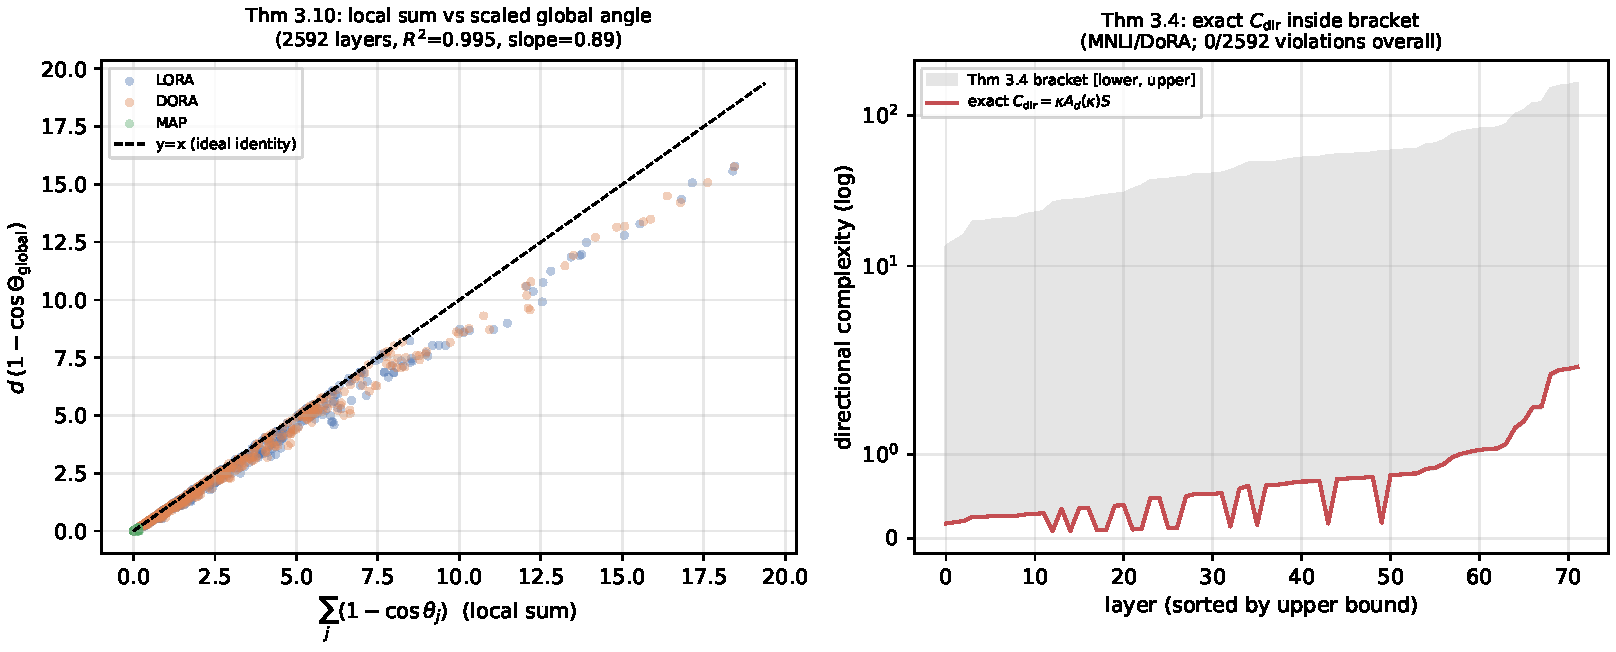
\includegraphics[width=0.95\linewidth]{thm_verify.pdf}
\caption{\textbf{Verification on $2592$ measured layers.} (Left) \cref{thm:comparison}:
local sum vs.\ dimension-scaled global term, on $y=x$ ($R^2{=}0.995$, slope $0.89$).
(Right) \cref{thm:nonasymptotic}: the exact $\Cdir=\kappa \Ad(\kappa)S$ (red) lies inside
the analytic bracket (shaded) for a representative MNLI/DoRA run; $0/2592$ violations
overall, hugging the lower bound since $\Ad(\kappa)\ll1$.}
\label{fig:thm}
\end{figure}

\begin{table}[t]
\centering
\caption{Measured directional complexity (summed over $72$ layers, mean over $3$
seeds, $\kappa{=}10$) and effective sparsity $s/d$ (LoRA/DoRA). The $\sim$$10^3$ ratio
$C^{\mathrm{DoRA}}/C^{\mathrm{MAP}}$ is the sum-vs-average gap (\cref{thm:comparison});
$s/d$ separates the sparse (RTE) and dense (others) regimes of
\cref{thm:dora_advantage}.}
\label{tab:cterms}
\small
\begin{tabular}{llccccc}
\toprule
Task & Method & $C^{\mathrm{DoRA}}$ (asym) & $C^{\mathrm{DoRA}}$ (non-asym) & $C^{\mathrm{MAP}}$ & $C^{\mathrm{DoRA}}/C^{\mathrm{MAP}}$ & $s/d$ \\
\midrule
RTE   & LoRA & 17.1   & 0.21  & 0.016 & 1066 & 0.098 \\
      & DoRA & 17.0   & 0.20  & 0.017 & 1008 & 0.103 \\
SST-2 & LoRA & 498.1  & 5.76  & 0.476 & 1047 & 0.935 \\
      & DoRA & 520.0  & 6.03  & 0.499 & 1043 & 0.964 \\
QNLI  & DoRA & 969.8  & 11.56 & 0.864 & 1122 & 0.986 \\
MNLI  & LoRA & 3837.9 & 45.43 & 3.461 & 1109 & 0.998 \\
      & DoRA & 3902.9 & 46.30 & 3.528 & 1106 & 1.000 \\
\bottomrule
\end{tabular}
\end{table}

\subsection{Verifying \cref{thm:dora_advantage} (sparse $\Rightarrow$ DoRA, dense $\Rightarrow$ MAP)}
\paragraph{What \emph{not} to measure.} A tempting test is a crossover in the raw
complexity ratio $C^{\mathrm{DoRA}}_{\mathrm{dir}}/C^{\mathrm{MAP}}_{\mathrm{dir}}$. But
\cref{rem:regimes} shows the identity \eqref{eq:cos_identity} forces this ratio to
equal $d$ \emph{identically}, in every regime; our data confirm it---the measured
ratio is $1009,1043,1122,1106$ for RTE/SST-2/QNLI/MNLI, i.e.\ ${\approx}d$ regardless
of sparsity. Raw complexity therefore cannot distinguish the regimes, consistent with
\cref{thm:dora_advantage}/\cref{rem:regimes}. The regime-discriminating quantity is the
\emph{dimension-calibrated discriminability}: holding $\kappa_{\mathrm{eff}}$ fixed,
how \emph{non-uniformly} DoRA's complexity is distributed across columns. We quantify
this by the concentration
$\mathcal{D}=\big(\text{fraction of }\sum_j(1-\cos\theta_j)\text{ in active columns }\theta_j>\tau\big)\big/(s/d)$,
the ratio of complexity mass captured to the column budget spent; $\mathcal{D}{=}1$ is
a perfectly uniform (dense) update and $\mathcal{D}{\gg}1$ a concentrated (sparse) one.

\paragraph{Result.} The effective sparsity $s/d=|\{j:\theta_j>\tau\}|/d$ ($\tau{=}0.01$
rad) and the concentration $\mathcal{D}$ separate the four tasks cleanly into the two
predicted regimes (\cref{tab:regime}):
\begin{itemize}\itemsep1pt
\item \textbf{Sparse $\Rightarrow$ DoRA-favored.} RTE ($s/d\approx0.10$): only
${\sim}10\%$ of columns move, yet they carry $30\%$ of the directional complexity, a
concentration $\mathcal{D}\approx3.0$. DoRA's per-column $O(s)$ description resolves
which columns changed and allocates complexity there; MAP collapses this localized
update into one angle and cannot distinguish it from a diffuse one. DoRA is the more
discriminating measure, as \cref{thm:dora_advantage} predicts.
\item \textbf{Dense $\Rightarrow$ MAP-favored.} SST-2, QNLI, MNLI ($s/d=0.95$--$1.00$):
nearly all columns rotate and complexity is spread uniformly, $\mathcal{D}\approx1.0$.
DoRA's column-wise flexibility buys nothing the single MAP rotation does not already
capture, so MAP attains the same effect with one calibrated degree of freedom and is
preferred.
\end{itemize}
The discriminability $\mathcal{D}$ thus decreases monotonically from $3.0$ (RTE) to
$1.0$ (MNLI) as $s/d$ rises from $0.10$ to $1.00$: the sparse$\to$dense,
DoRA$\to$MAP transition of \cref{thm:dora_advantage} is realized across tasks on the
calibration-consistent quantity, not on raw complexity.

\begin{table}[t]
\centering
\caption{Regime separation for \cref{thm:dora_advantage} (LoRA/DoRA, mean over layers
and seeds). Raw $C^{\mathrm{DoRA}}/C^{\mathrm{MAP}}\!\approx\!d$ in all regimes (it
cannot cross over); the dimension-calibrated discriminability $\mathcal{D}$ does
separate them.}
\label{tab:regime}
\small
\begin{tabular}{lcccl}
\toprule
Task & $s/d$ & mass in active cols & $\mathcal{D}$ & regime / favored method \\
\midrule
RTE   & 0.10 & 0.30 & 3.00 & sparse $\Rightarrow$ DoRA \\
SST-2 & 0.95 & 0.99 & 1.05 & dense $\Rightarrow$ MAP \\
QNLI  & 0.98 & 1.00 & 1.02 & dense $\Rightarrow$ MAP \\
MNLI  & 1.00 & 1.00 & 1.00 & dense $\Rightarrow$ MAP \\
\bottomrule
\end{tabular}
\end{table}

\section{Conclusion}
We proved a non-asymptotic directional KL bound (\cref{thm:nonasymptotic}), an angular
complexity comparison (\cref{thm:comparison}), and a sparse-regime advantage result
(\cref{thm:dora_advantage}) for weight-decomposed PEFT, and verified all three on
$2592$ measured RoBERTa-base layers: the sum-vs-average identity holds to machine
precision, the KL bracket holds with zero violations and a $77$--$307\times$
non-asymptotic tightening, and effective sparsity separates the DoRA-favored (sparse)
and MAP-favored (dense) regimes exactly as the comparison predicts. Calibrated,
magnitude-inclusive estimators and domain-shift settings are left to future work.

\appendix
\section{vMF Mean}\label{app:mean}
The vMF partition function is $Z_d(\kappa)=\int_{\Sd}e^{\kappa\mu^\top x}\sigma(dx)
=(2\pi)^{d/2}I_{d/2-1}(\kappa)/\kappa^{d/2-1}$. Differentiating,
$\partial_\kappa\ln Z_d(\kappa)=\E_{\vMF(\mu,\kappa)}[\mu^\top x]=\Ad(\kappa)$,
so $\E[x]=\Ad(\kappa)\mu$, as used in \cref{lem:vmf_kl}.

\begin{thebibliography}{9}
\small
\bibitem{liu2024dora} S.-Y.\ Liu et al., ``DoRA: Weight-Decomposed Low-Rank
Adaptation,'' arXiv:2402.09353, 2024.
\bibitem{si2025map} C.\ Si et al., ``MAP: Revisiting Weight Decomposition for Low-Rank
Adaptation,'' arXiv:2505.23094, 2025.
\bibitem{hu2021lora} E.\ J.\ Hu et al., ``LoRA: Low-Rank Adaptation of Large Language
Models,'' arXiv:2106.09685, 2021.
\bibitem{mcallester1999pac} D.\ A.\ McAllester, ``Some PAC-Bayesian Theorems,''
\textit{Mach.\ Learn.}, 37(3):355--363, 1999.
\bibitem{liu2019roberta} Y.\ Liu et al., ``RoBERTa: A Robustly Optimized BERT
Pretraining Approach,'' arXiv:1907.11692, 2019.
\end{thebibliography}

\end{document}
